\section{Tiền xử lý dữ liệu}
Dữ liệu gốc chứa gần 1,5 triệu bản ghi các dữ liệu đều đã được mã hóa dưới dạng số. Tha thực hiện ETL dữ liệu bằng Excel  gồm các thao tác như thay thế giá trị , đổi kiểu dữ liệu , tách cột , xử lý các cột ngày tháng 
Đầu tiên đưa dữ liệu vào Power query .Nhận thấy có 3 file dữ liệu của năm 2013 , 2014, 2015 đều có các cột tương ứng giống nhau . Để giúp cho việc thống kê và báo cáo được dễ dàng hơn  ta thực hiện nối các bảng lại với nhau bằng cách sử dụng \textbf{Append Quieries } .
\\\textbf{Xử lý dữ liệu mã hóa }
Các dữ liệu trong bảng 2013, 2014,2015 đều đã được mã hóa dưới dạng số. Do đó cần phải giải mã chúng để đưa về các giá trị cụ thể chi tiết hơn. Có rất nhiều cách để giải mã như tách cột, thêm cột, thêm cột có
điều kiện, thay thế giá trị, .... Cụ thể:
\begin{itemize}
    \item Giải mã dữ liệu cột IDAY , IMOUNTH , IYEAR \\\hfill
    Nhận thấy dữ liệu trong các cột IDAY, IMOUTH ,IYEAR đều được bao bọc bởi cặp dấu \textbf{''} do đó cần phải tách dữ liệu ra bằng cách xử dụng \textbf{Split Column } với dấu phân cách là \textbf{'}. Ta thu được kết quả như hình dưới :
    
            \begin{figure}[!h]
                \begin{center}
                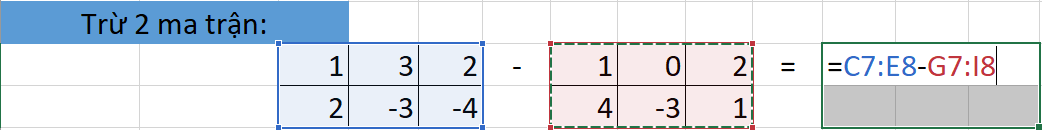
\includegraphics[scale = 0.8]{HONG/2.png}
              \caption{Khảo sát về khả năng tiếp cận y tế}
         
\end{center}
   \end{figure}
   Sau khi đã tách dữ liệu của 3 cột ta thực hiện xóa các cột IMONTH.1,IMONTH.3 , IYEAR.1 ,IYEAR.3 ,IDAY.1 ,IDAY.3 bởi vì các cột này đều không có giá trị sử dụng . Thực hiện gộp các cột IDAY.2 , IMONTH.2 ,IYEAR.2    với nhau bằng cách sử dụng\textit{ merge columns} với seperator là / , sau đó chuyển dữ liệu về dạng ngày tháng ta thu được kết quả như hình dưới đây :
    \begin{figure}[!h]
                \begin{center}
                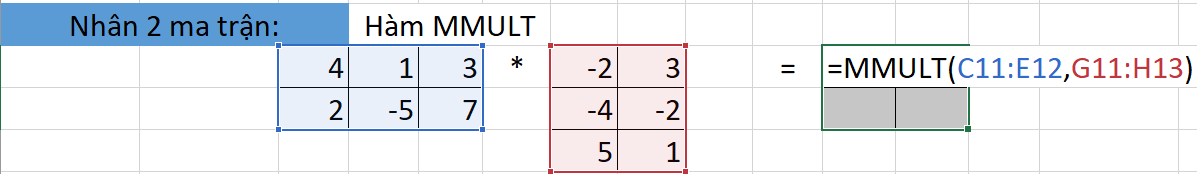
\includegraphics[scale = 0.8]{HONG/3.png}
              \caption{Khảo sát về khả năng tiếp cận y tế}
         
\end{center}
   \end{figure}
   \item Giải mã hóa các cột giá trị khác 
   Thực hiện thay thế các giá trị số thành các giá trị cụ thể ví dụ như ở cột \textbf{SEX} chỉ có 2 giá trị số là 1 và 2 , nhìn vào giá trị ta không thể biết được nó có nghĩa là gì do đó ta cần giải mã nó với 1 tương ứng là\textit{ male} , với 2 tương ứng là\textit{ female }.
   Thực hiện giải mã bằng cách thay thế giá trị (sử dụng replace values ) hoặc megre quieres bảng gốc với bảng dữ liệu giải mã tương ứng . Tuy nhiên khi dữ liệu bị mã hóa có nhiều việc thay thế giá trị sẽ rất là tốn thời gian do đó ta thực hiện merge quieres thu được kết quả như hình dưới
     \begin{figure}[!h]
                \begin{center}
                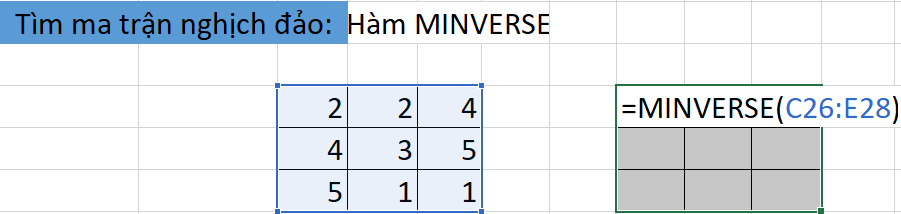
\includegraphics[scale = 0.8]{HONG/5.png}
                \end{center}
    \end{figure}
\end{itemize}
\textbf{Xóa các giá trị null trong bảng }
Thực hiện xóa các giá trị null ở mỗi bảng .Các giá trị này sẽ làm cho việc báo cáo thống kê phức  tạp do đó ta cần thực thao tác xóa . Dưới đây là kết quả của quá trình xóa các giá trị null trong cột \textbf{LASTSMK2} :
 
            \begin{figure}[!h]
                \begin{center}
                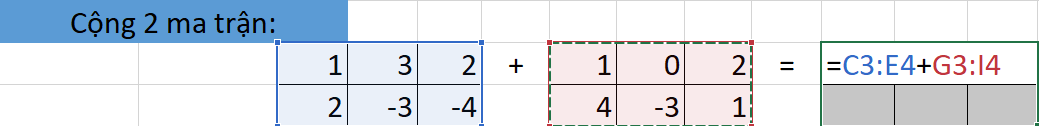
\includegraphics[scale = 0.8]{HONG/1.png}
              \caption{Khảo sát về khả năng tiếp cận y tế}
         
\end{center}
   \end{figure}
\begin{itemize}
\item Tách các sheet theo từng chủ đề :

\begin{itemize}
    \item PeopleInfor: Thông tin cá nhân của người tham gia khảo sát.
    \item PeopleHealth: Tình trạng sức khỏe của người tham gia khảo sát.
\item SmokeStatus: Tình trạng hút thuốc của người tham gia khảo sát.
\item Date: Ngày khảo sát.
\end{itemize} 
\item Xử lí dữ liệu mã hóa: Sử dụng các công cụ như tách cột, thêm cột, thêm cột có
điều kiện, thay thế giá trị, ... để thay các giá trị mã hóa thành các thông tin có ý
nghĩa.
\item Các dữ liệu bị mã hóa có nhiều hơn 5 giá trị được thống kê thành các bảng thông
tin.
\end{itemize}
Lưu dữ liệu vào cơ sở dữ liệu:

\begin{itemize}
    \item Dữ liệu sau khi được xử lí đơn giản được lưu vào CSDL HealthCare, vùng dữ liệu
được lưu này gọi là Stagging, là vùng đệm chứa dữ liệu trước khi đưa vào kho dữ liệu.
\item Xây dựng kho dữ liệu bằng cách tạo các bảng trong cơ sở dữ liệu theo mô hình OLAP
đã được thiết kế.

\end{itemize}
Đổ dữ liệu từ cơ sở dữ liệu vào kho dữ liệu:
\begin{itemize}
    \item Các dữ liệu cố định, không thay đổi theo thời gian sẽ được chuyển trực tiếp từ
Stagging vào Kho dữ liệu thông qua câu lệnh “Insert”
\item Đối với các dữ liệu được cập nhật định kì theo thời gian (tức là cứ sau một khoảng
thời gian sẽ có dữ liệu) mới được thêm vào thì việc cứ mỗi lần phải viết lại câu lệnh
“Insert” là rất mất thời gian. Thay vào đó, ta sẽ đưa câu lệnh “Insert” tạo thành một
thủ tục để mỗi lần cập nhật dữ liệu ta chỉ cần gọi thủ thục một cách nhanh chóng.
\begin{itemize}
    \item Thủ tục đổ dữ liệu vào các bảng Dim
\end{itemize} 
\end{itemize}
